\section{Theoretical background}
\label{sec:background}

\subsection{Data sets}
\label{subsec:Datasets}

\begin{figure}[h!]
\centering
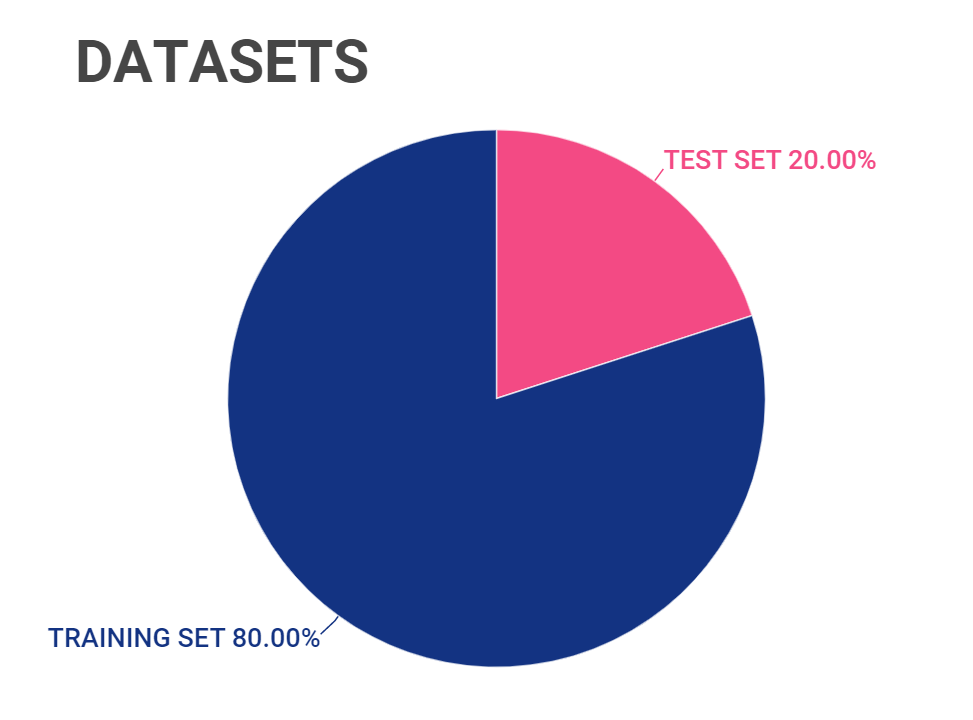
\includegraphics[scale=0.45]{Images/2_theory/datasets.PNG}
\caption{Division of data sets}
\label{fig:datasets}
\end{figure}

\subsection{Feature engineering}
\label{subsec:feature_eng}
Feature engineering is the process of improving predictive modelling performance on data set through data mining techniques. This is done by a process called feature extraction, where relevant features are extracted from the raw data, and thereby transforming the feature space. A feature is defined as an individual measurable property or characteristic of an observed phenomenon or event. Feature space is defined as a collection of features that characterize the data set \cite{Bishop}.

\todo[inline, color=orange!40]
{
define test set, training set. Relate to error and empirical risk of classifier.A Probabilistic Theory of Pattern Recognition 4.5 virker relevant. Link to the pareto principle.

    -datasets
    -error
    -underfitting/overfitting
    -data mining
    -feature engineering
    -surrogate models
    
    Relevant litterature: Feature Selection for Knowledge Discovery and Data Mining
    
    
    \vspace{0.2cm}
}